\documentclass[border=12pt]{standalone}
\def\pgfsysdriver{pgfsys-dvisvgm.def}
\usepackage[dvisvgm]{xcolor}
\usepackage{xeCJK}
\setCJKmainfont{HaranoAjiGothic-Regular.otf}[BoldFont=HaranoAjiGothic-Bold.otf]
\setCJKsansfont{HaranoAjiGothic-Regular.otf}[BoldFont=HaranoAjiGothic-Bold.otf]
\usepackage{amsmath,amssymb,tikz,lmodern}
\usetikzlibrary{arrows.meta,positioning,calc,fit,backgrounds}
\renewcommand{\familydefault}{\sfdefault}
\definecolor{ink}{HTML}{25322F}
\definecolor{green}{HTML}{246657}
\definecolor{tint}{HTML}{EEF4F0}
\definecolor{soft}{HTML}{C6D2CC}
\definecolor{muted}{HTML}{52615B}
\newif\ifJapanese
\newcommand{\Tx}[2]{\ifJapanese #1\else #2\fi}
\newcommand{\Eff}{\overline{\operatorname{Eff}}}
\newcommand{\heading}[3]{{\color{green}\bfseries #1\quad\Tx{#2}{#3}}\\[5pt]}
% A white rectangle makes the complete citation label clickable, including spaces.
\newcommand{\refurl}[2]{\special{dvisvgm:raw <a xlink:href="#1" target="_blank" rel="noopener noreferrer">}{\setlength{\fboxsep}{0pt}\colorbox{white}{\color{green}\underline{\strut #2}}}\special{dvisvgm:raw </a>}}
\tikzset{
 card/.style={draw=soft,fill=white,rounded corners=2pt,align=left,text=ink,font=\fontsize{10.5}{14}\selectfont,inner xsep=12pt,inner ysep=10pt,text width=14.4cm},
 half/.style={card,text width=6.45cm,minimum height=2.05cm},
 result/.style={card,draw=green,fill=tint,line width=.9pt},
 reason/.style={align=left,text=muted,font=\fontsize{9}{12}\selectfont,inner sep=0pt,text width=12.7cm},
 branchreason/.style={reason,text width=5.95cm},
 edge/.style={-{Stealth[length=2.4mm]},draw=green,line width=1pt},
 wire/.style={draw=green,line width=1pt},
}
% Keep the arrow in a dedicated left gutter; explanations never cover it.
\newcommand{\flow}[3]{
 \coordinate (#2-from) at ($(#1.south)+(-6.9,0)$);
 \coordinate (#2-to) at ($(#2.north)+(-6.9,0)$);
 \draw[edge] (#2-from)--(#2-to);
 \node[reason,anchor=west] (#2-reason) at ($(#2-from)!.5!(#2-to)+(.55,0)$) {#3};
}

\newcommand{\Cite}[2]{\refurl{#1}{#2}}

\Japanesetrue
\begin{document}
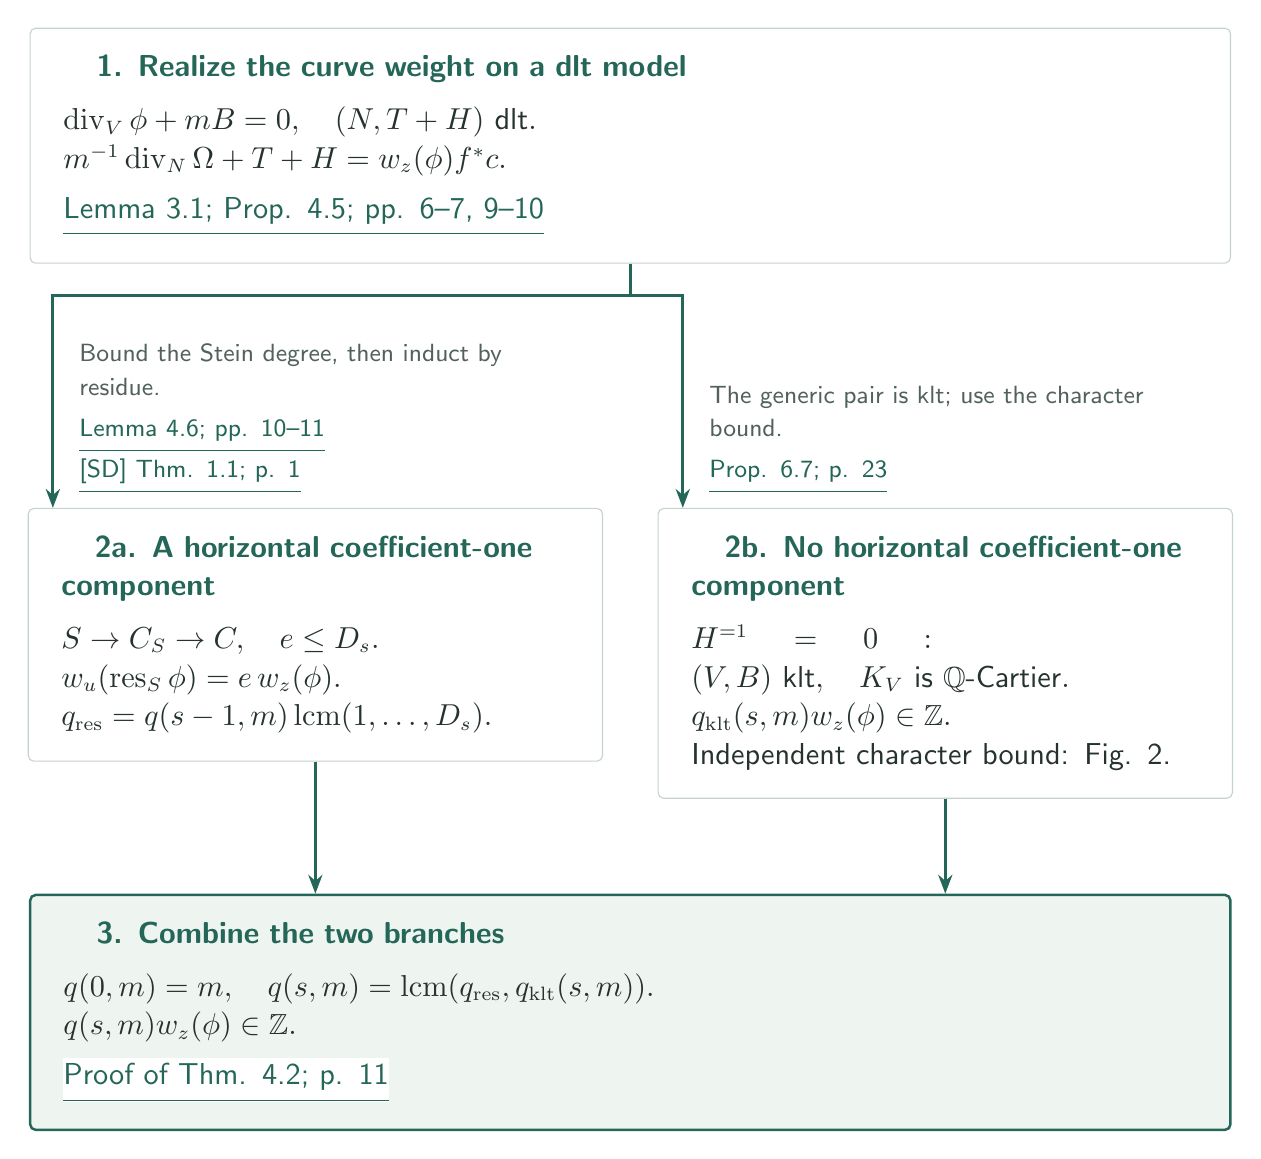
\begin{tikzpicture}
\node[card] (weight) {\heading{}{1. 曲線重みをdltモデルに載せる}{1. Realize the curve weight on a dlt model}$\operatorname{div}_V\phi+mB=0,\quad (N,T+H)\text{ dlt}.$\\ $m^{-1}\operatorname{div}_N\Omega+T+H=w_z(\phi)f^*c.$\\[4pt]\Cite{https://github.com/openai/math/blob/adc7f1241b42e322a6451854ab7e4b4c146bf78a/preprints/Uniform-log-Iitaka-fibrations-and-bounded-moduli-denominators-October-4-2026/uniform-log-iitaka.pdf}{Lemma 3.1; Prop. 4.5; pp. 6--7, 9--10}};

\node[half,below=3.1cm of weight.south,xshift=-4cm] (lc) {\heading{}{2a. 水平係数1成分がある}{2a. A horizontal coefficient-one component}$S\to C_S\to C,\quad e\le D_s.$\\ $w_u(\operatorname{res}_S\phi)=e\,w_z(\phi).$\\ $q_{\rm res}=q(s-1,m)\operatorname{lcm}(1,\ldots,D_s).$};

\node[half,below=3.1cm of weight.south,xshift=4cm] (klt) {\heading{}{2b. 水平係数1成分がない}{2b. No horizontal coefficient-one component}$H^{=1}=0:\quad (V,B)\text{ klt},\quad K_V\text{ is }\mathbb Q\text{-Cartier}.$\\ $q_{\rm klt}(s,m)w_z(\phi)\in\mathbb Z.$\\ \Tx{独立な指標評価は第2図。}{Independent character bound: Fig. 2.}};

\coordinate (lc-a) at ($(lc.north west)+(.32,0)$);
\draw[edge] (weight.south) -- ++(0,-.4) -| (lc-a);
\node[branchreason,anchor=south west] at ($(lc.north west)+(.65,.18)$) {\Tx{Stein次数を抑えて留数へ帰納。}{Bound the Stein degree, then induct by residue.}\\[3pt]\Cite{https://github.com/openai/math/blob/adc7f1241b42e322a6451854ab7e4b4c146bf78a/preprints/Uniform-log-Iitaka-fibrations-and-bounded-moduli-denominators-October-4-2026/uniform-log-iitaka.pdf}{Lemma 4.6; pp. 10--11}\\ \Cite{https://github.com/openai/math/blob/adc7f1241b42e322a6451854ab7e4b4c146bf78a/preprints/Arithmetic-Stein-degree-bounds-for-log-Calabi-Yau-pairs-September-25-2026/paper.pdf}{[SD] Thm. 1.1; p. 1}};

\coordinate (klt-a) at ($(klt.north west)+(.32,0)$);
\draw[edge] (weight.south) -- ++(0,-.4) -| (klt-a);
\node[branchreason,anchor=south west] at ($(klt.north west)+(.65,.18)$) {\Tx{一般対がkltとなるので指標評価を使う。}{The generic pair is klt; use the character bound.}\\[3pt]\Cite{https://github.com/openai/math/blob/adc7f1241b42e322a6451854ab7e4b4c146bf78a/preprints/Uniform-log-Iitaka-fibrations-and-bounded-moduli-denominators-October-4-2026/uniform-log-iitaka.pdf}{Prop. 6.7; p. 23}};

\node[result,below=8cm of weight.south] (end) {\heading{}{3. 二つの枝を合わせる}{3. Combine the two branches}$q(0,m)=m,\quad q(s,m)=\operatorname{lcm}(q_{\rm res},q_{\rm klt}(s,m)).$\\ $q(s,m)w_z(\phi)\in\mathbb Z.$\\[4pt]\Cite{https://github.com/openai/math/blob/adc7f1241b42e322a6451854ab7e4b4c146bf78a/preprints/Uniform-log-Iitaka-fibrations-and-bounded-moduli-denominators-October-4-2026/uniform-log-iitaka.pdf}{Proof of Thm. 4.2; p. 11}};

\draw[edge] (lc.south) -- ++(0,-.5) -| ($(end.north)+(-4,0)$);
\draw[edge] (klt.south) -- ++(0,-.5) -| ($(end.north)+(4,0)$);
\end{tikzpicture}
\end{document}
